\documentclass{article}

\usepackage{fancyhdr}
\usepackage{extramarks}
\usepackage{amsmath}
\usepackage{amsthm}
\usepackage{amsfonts}
\usepackage{tikz}
\usepackage[plain]{algorithm}
\usepackage{algpseudocode}
\usepackage{graphicx}
\usetikzlibrary{automata,positioning}
\usepackage{listings}

%
% Basic Document Settings
%

\topmargin=-0.45in
\evensidemargin=0in
\oddsidemargin=0in
\textwidth=6.5in
\textheight=9.0in
\headsep=0.25in

\linespread{1.1}

\pagestyle{fancy}
\lhead{\hmwkAuthorName}
\chead{\hmwkClass\ : \hmwkTitle}
\rhead{\firstxmark}
\lfoot{\lastxmark}
\cfoot{\thepage}

\renewcommand\headrulewidth{0.4pt}
\renewcommand\footrulewidth{0.4pt}

\setlength\parindent{0pt}

%
% Create Problem Sections
%

\newcommand{\enterProblemHeader}[1]{
    \nobreak\extramarks{}{Problem \arabic{#1} continued on next page\ldots}\nobreak{}
    \nobreak\extramarks{Problem \arabic{#1} (continued)}{Problem \arabic{#1} continued on next page\ldots}\nobreak{}
}

\newcommand{\exitProblemHeader}[1]{
    \nobreak\extramarks{Problem \arabic{#1} (continued)}{Problem \arabic{#1} continued on next page\ldots}\nobreak{}
    \stepcounter{#1}
    \nobreak\extramarks{Problem \arabic{#1}}{}\nobreak{}
}

\setcounter{secnumdepth}{0}
\newcounter{partCounter}
\newcounter{homeworkProblemCounter}
\setcounter{homeworkProblemCounter}{1}
\nobreak\extramarks{Problem \arabic{homeworkProblemCounter}}{}\nobreak{}

%
% Homework Problem Environment
%
% This environment takes an optional argument. When given, it will adjust the
% problem counter. This is useful for when the problems given for your
% assignment aren't sequential. See the last 3 problems of this template for an
% example.
%
\newenvironment{homeworkProblem}[1][-1]{
    \ifnum#1>0
        \setcounter{homeworkProblemCounter}{#1}
    \fi
    \section{Problem \arabic{homeworkProblemCounter}}
    \setcounter{partCounter}{1}
    \enterProblemHeader{homeworkProblemCounter}
}{
    \exitProblemHeader{homeworkProblemCounter}
}

%
% Homework Details
%   - Title
%   - Due date
%   - Class
%   - Section/Time
%   - Instructor
%   - Author
%

\newcommand{\hmwkTitle}{Homework\ \#3 }
\newcommand{\hmwkDueDate}{April 12, 2018}
\newcommand{\hmwkClass}{BMI 776}
\newcommand{\hmwkClassTime}{}
\newcommand{\hmwkClassInstructor}{}
\newcommand{\hmwkAuthorName}{\textbf{John Steill}}
%\and \textbf{Davis Josh}}

%
% Title Page
%

\title{
    \vspace{2in}
    \textmd{\textbf{\hmwkClass:\ \hmwkTitle}}\\
    \normalsize\vspace{0.1in}\small{Due\ on\ \hmwkDueDate\ at 3:10pm}\\
    \vspace{0.1in}\large{\textit{\hmwkClassInstructor\ \hmwkClassTime}}
    \vspace{3in}
}

\author{\hmwkAuthorName}
\date{}

\renewcommand{\part}[1]{\textbf{\large Part \Alph{partCounter}}\stepcounter{partCounter}\\}

%
% Various Helper Commands
%

% Useful for algorithms
\newcommand{\alg}[1]{\textsc{\bfseries \footnotesize #1}}

% For derivatives
\newcommand{\deriv}[1]{\frac{\mathrm{d}}{\mathrm{d}x} (#1)}

% For partial derivatives
\newcommand{\pderiv}[2]{\frac{\partial}{\partial #1} (#2)}

% Integral dx
\newcommand{\dx}{\mathrm{d}x}

% Alias for the Solution section header
\newcommand{\solution}{\textbf{\large Solution}}

% Probability commands: Expectation, Variance, Covariance, Bias
\newcommand{\E}{\mathrm{E}}
\newcommand{\Var}{\mathrm{Var}}
\newcommand{\Cov}{\mathrm{Cov}}
\newcommand{\Bias}{\mathrm{Bias}}

\begin{document}

%\maketitle

\pagebreak

\begin{homeworkProblem}
\textbf{1A Dragonn: Training convolutional networks}

\begin{itemize}
	\item{\textbf{1-layer training}
	\begin{itemize}
		\item{At the first epoch, the training auPRC was .511, and the validation auPRC was .526.}
		\item{At the final epoch, the training auPRC was .577 and the validation auPRC was .516.}
	\end{itemize}}
	\item{\textbf{2-layer training}
	\begin{itemize}
		\item{}
		\item{}
	\end{itemize}}
\end{itemize}





%%%%%%%%%%%%%%%%%%%%%%%%%%%%%%%%%%%%%%%%%%
\textbf{1B: Using and interpreting trained convolutional networks}
\begin{itemize}
	\item{\textbf{Input and output dimensions of the first Convolution2D layer} The input dimensions, 4 and 500, correspond to the 4 character, 500 base length input sequences.  The output dimensions, 1 and 486, correspond to the 15-base convolution outputs. Position domains begin with (1,15) and continue to (486,500). }
	\item{\textbf{Input and output dimensions of the Dense layer}. The input layer dimension, 195, arises from the number of nodes in all the previous "flatten" layer, 15 by 13. The output dimension of 1 corresponds to the NN's estimate of the probability of a positive condition given the input.}
	\item{\textbf{Test Confusion Matrix} \vspace{3 mm} \\ 
		\begin{tabular}{|| l l ||} 
			\hline
			\multicolumn{2}{|c|}{2-Layer Test Results} \\I:I
			\hline
			positive\_test\_0	& P(bound)=0.897705674171 \\
			positive\_test\_1	& P(bound)=0.925364196301 \\
			positive\_test\_2	& P(bound)=0.806158542633 \\
			positive\_test\_3	& P(bound)=0.909259021282 \\
			positive\_test\_4	& P(bound)=0.490884274244 \\
			\hline
			negative\_test\_0 & P(bound)=0.708925485611 \\
			negative\_test\_1 & P(bound)=0.161382764578 \\the:W
			negative\_test\_2 & P(bound)=0.941750407219 \\
			negative\_test\_3 & P(bound)=0.781042456627 \\
			negative\_test\_4 & P(bound)=0.526986956596 \\
			\hline
		\end{tabular}
 		\hspace{3 mm}
 		\begin{tabular}{|| l l ||} 
 			\hline
 			True Positives & 4 \\
 			False Positives  & 4 \\
			 True Negatives & 1 \\
 			False Negatives & 1 \\
			 \hline
		\end{tabular}  }
	\item{\textbf{Filters vs Final Motifs} The filters do not obviously resemble the final motifs. This is not surprising. Filters are different objects, for example they ave both positive and negative values. The are optimized to be used in conjunction with each other in the next neural net. The can detect interaction effects between nearby position, where PWMs assume strict information independence.}
	\item{\textbf{DeepLIFT scores}}
\end{itemize}


\end{homeworkProblem}
%\newpage
%\begin{homeworkProblem}
%\textbf{2A  Probabilities in the Markov random field}
%\begin{itemize}
%	\item{How many possible configurations are there in this network?  $2^{15} = 32768$}
%	\item{What are the most probable and the least probable configurations?}
%	\begin{itemize}
%		\item{The most probable configurations are when all nodes are in the same state: either on or off.}
%		\item{The least probable state is when nodes alternate between rows, so every pair is $(1,-1)$.}
%	\end{itemize} 
%	\item{Is it true that $P(R=1|S=1) = P(S=1|R=1)$?}
%	\begin{itemize}
%		\item{No it is not. For the $P(S=1|R=1)$ case, we note that the calculation is unaffected by the state of the left branch of the tree, which is "shielded" by the given $R$ state.}
%		\item{Because $S$ is a leaf node, in the $ P(R=1|S=1)$ case, the entire tree is still influencing $R$.}
%		\item{Therefore, $P(S=1|R=1) > P(R=1|S=1) $.}
%	\end{itemize} 
%\end{itemize}
%
%\textbf{2B: Gibbs sampling in the Markov random field}
%Here we program a gibbs sample, and estimate the probability of $P(R=1|S=1)$.
%Three iterations give values of .522, .528, and .547.  
%
%(To verify my answer to question 3 in part A, I estimated $P(S=1|R=1)$ to be about .55.)
%
%\end{homeworkProblem}
%
%\newpage
%\begin{homeworkProblem}
%\textbf{3A Estimating $\lambda$}
%Visually estimating $\lambda$ is tricky because choosing the flattest part motivates 
%$p > .6$: $$\frac{4 * 1750}{.4 * 20000} \approx  .85 $$ 
%However, I don't like this solution because the ideal curve is monotonically decreasing, if lambda was so high, there shouldn;t be so few 
%p-values in the $(.2,.6)$ range. Therefore I would choose the bumpier ride of a threshold of $p=.2$.
%$$\frac{8 * 1550}{.8 * 20000} \approx  .78$$ In any case, as we are only asked to approximate to the nearest tenth, I'm rounding down to 
%$$\lambda = .8 $$
%
%
%\textbf{3B Estimating $\hat{\pi}_0(\lambda)$}
%\begin{center}
% \begin{tabular}{|| c c c ||} 
%
% \hline
% $\lambda$ & $p_i > \lambda $ & $ \hat{\pi}_0(\lambda)$ \\ [0.5ex] 
%  \hline 
%  0.0 & 20000 & 1.00 \\
%0.1 & 15427 & 0.86 \\
%0.2 & 12893 & 0.81 \\
%0.3 & 11382 & 0.81 \\
%0.4 & 9834 & 0.82 \\
%0.5 & 8466 & 0.85 \\
%0.6 & 7030 & 0.88 \\
%0.7 & 5259 & 0.88 \\
%0.8 & 3484 & 0.87 \\
%0.9 & 1714 & 0.86 \\[1ex] 
%\hline
%\end{tabular} 
%\\[1.5ex]
%
%\end{center}
%
%\textbf{3C: Calculating q-values}
%\begin{center}
% \begin{tabular}{|| c c c ||} 
%\hline
%Rank & p-value & q-value \\ [0.5ex] 
%\hline
%0 & 0.000003 & 0.048 \\
%1 & 0.000007 & 0.056 \\
%2 & 0.000013 & 0.069 \\
%3 & 0.000024 & 0.088 \\
%4 & 0.000028 & 0.088 \\
%5 & 0.000033 & 0.088 \\
%6 & 0.000046 & 0.105 \\
%7 & 0.000055 & 0.110 \\
%8 & 0.000096 & 0.158 \\
%9 & 0.000099 & 0.158 \\
%\hline
%\end{tabular} 
%\\[1.5ex]
%
%\end{center}
%\end{homeworkProblem} 
%
%With a 2-layer training:
%\begin{itemize}
%	\item{\textbf{numpy.histogram2d(x,y,bins)} "Compute the bi-dimensional histogram of two data samples." }
%	\item{\textbf{chi2\_contingency(observed, correction, lambda\_)} "Chi-square test of independence of variables in a contingency table"}
%	\begin{itemize}
%		\item{Set lambda\_="log-likelihood"}
%		\item{The G-test statistic is proportional to the Kullback-Leibler divergence, by a factor of $2N$}
%		\item{Convert from nats to bits}
%		\item{\texttt{MI[gene\_a,gene\_b] = 0.5 * g / discrete\_expr.sum() / np.log(2)}}
%	\end{itemize}
%\end{itemize}
%
%\textbf{B. Equal Density Binning}
%
%The coded solution is in CalcMI.py.
%
%\textbf{C. Kernel Density Estimation}
%
%The coded solution is in CalcMI.py.
%
%\textbf{D. ROC plotting}
%
%The coded solution in included in plot.py
%
%\textbf{Prediction Evaluation}
%
%We are to evaluate several cases, and describe which gives the greatest AUROC.
%For the ones given, the 7-bin uniform density does best with an AUROC of .662 . 
%
%\begin{figure}[h!]
%\caption{7 bins, Uniform Size}
% 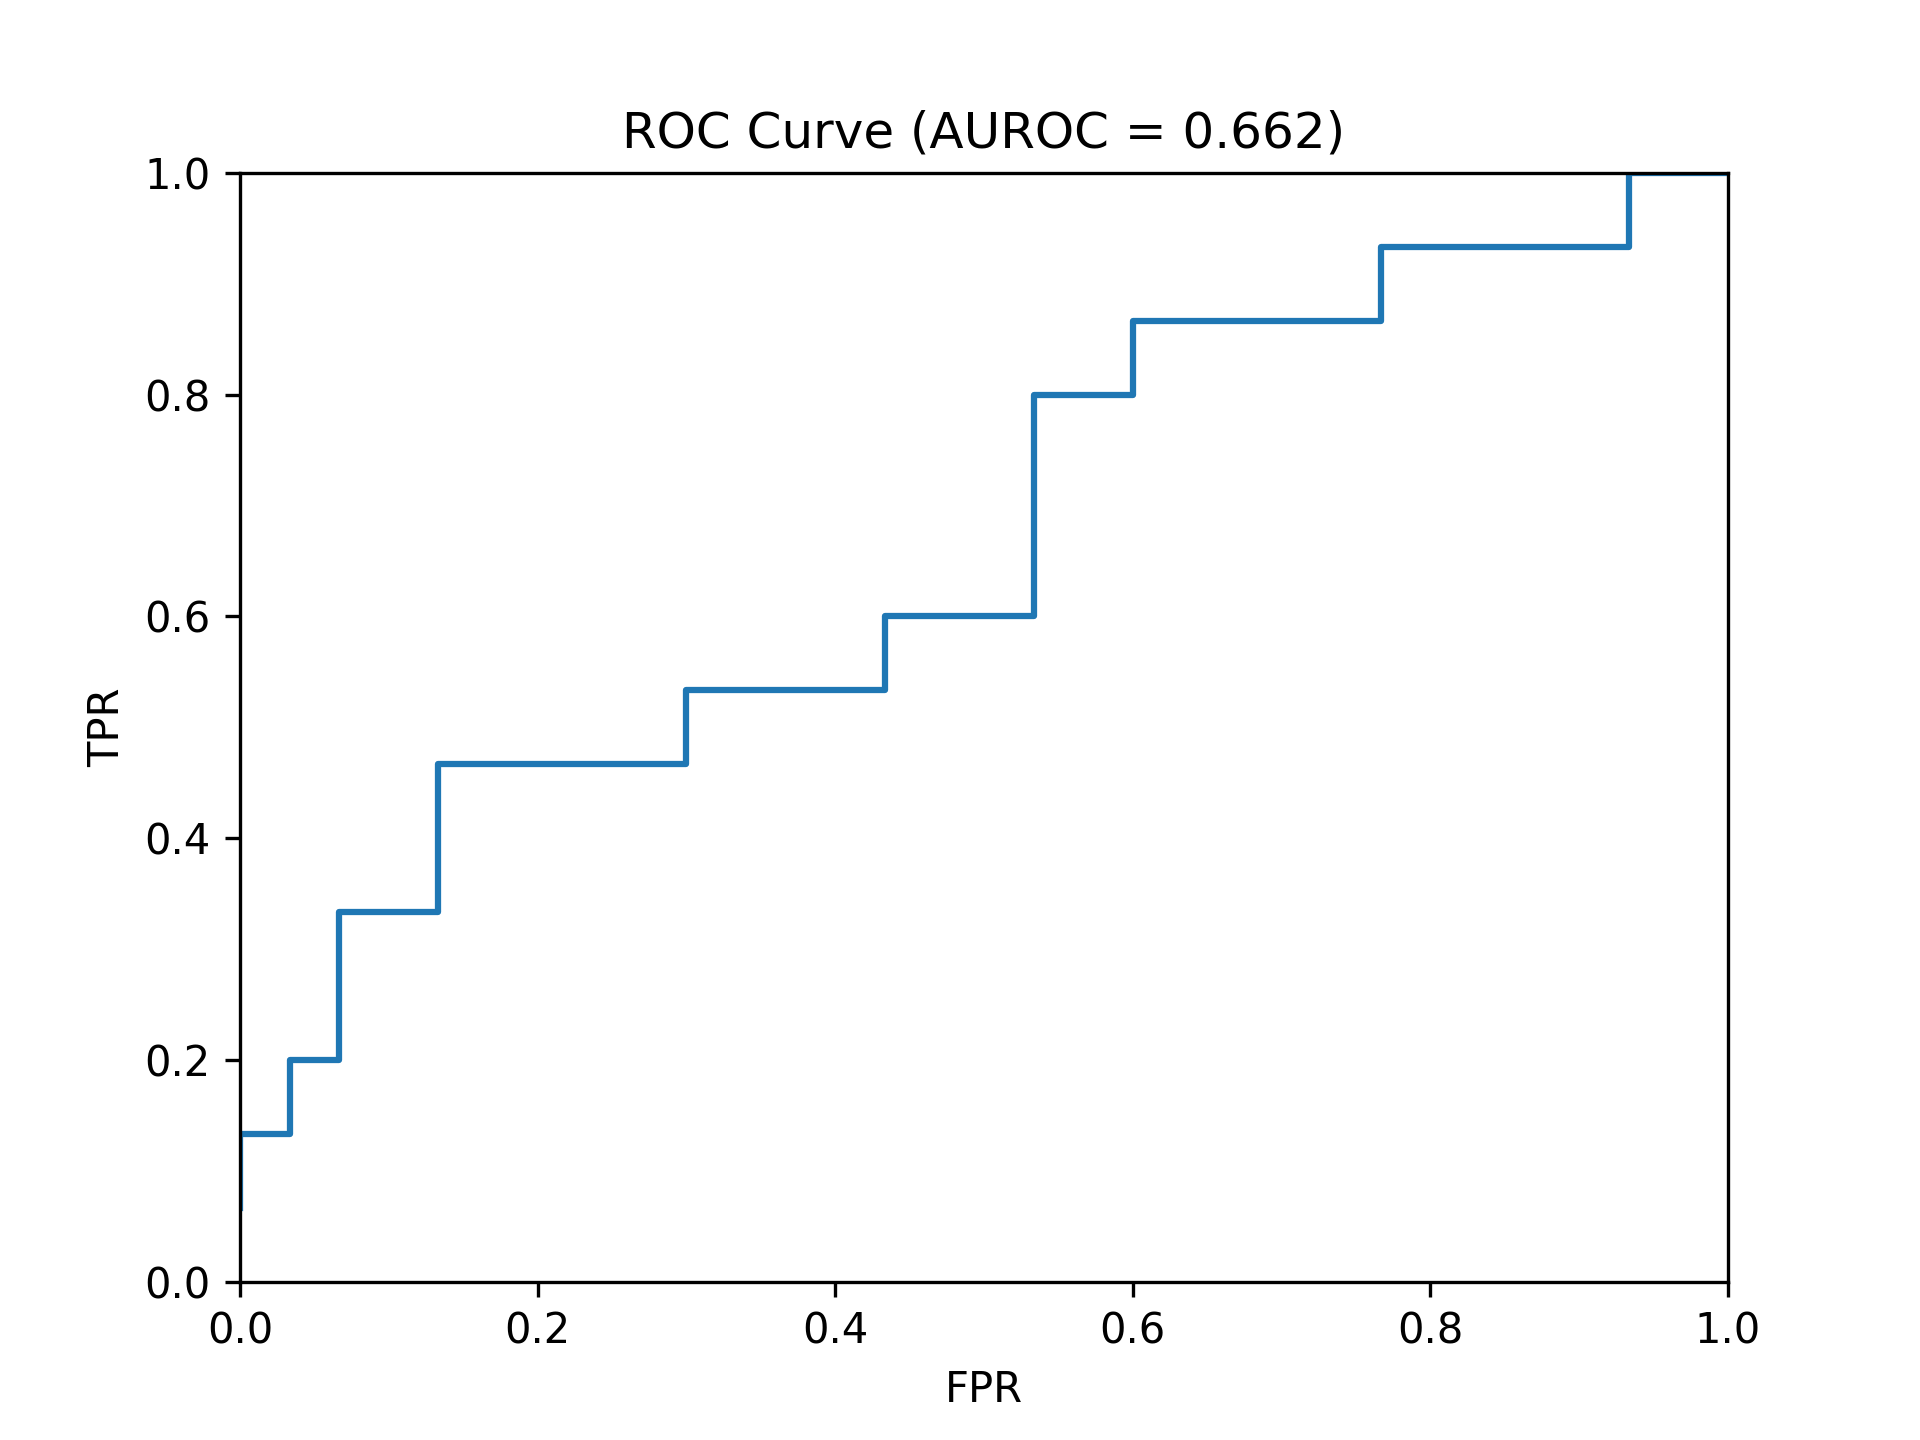
\includegraphics[width=3in]{uni_7b.png} 
% \centering
% \end{figure}
%
%\begin{figure}[h!]
%\caption{9 bins, Equal Density}
% 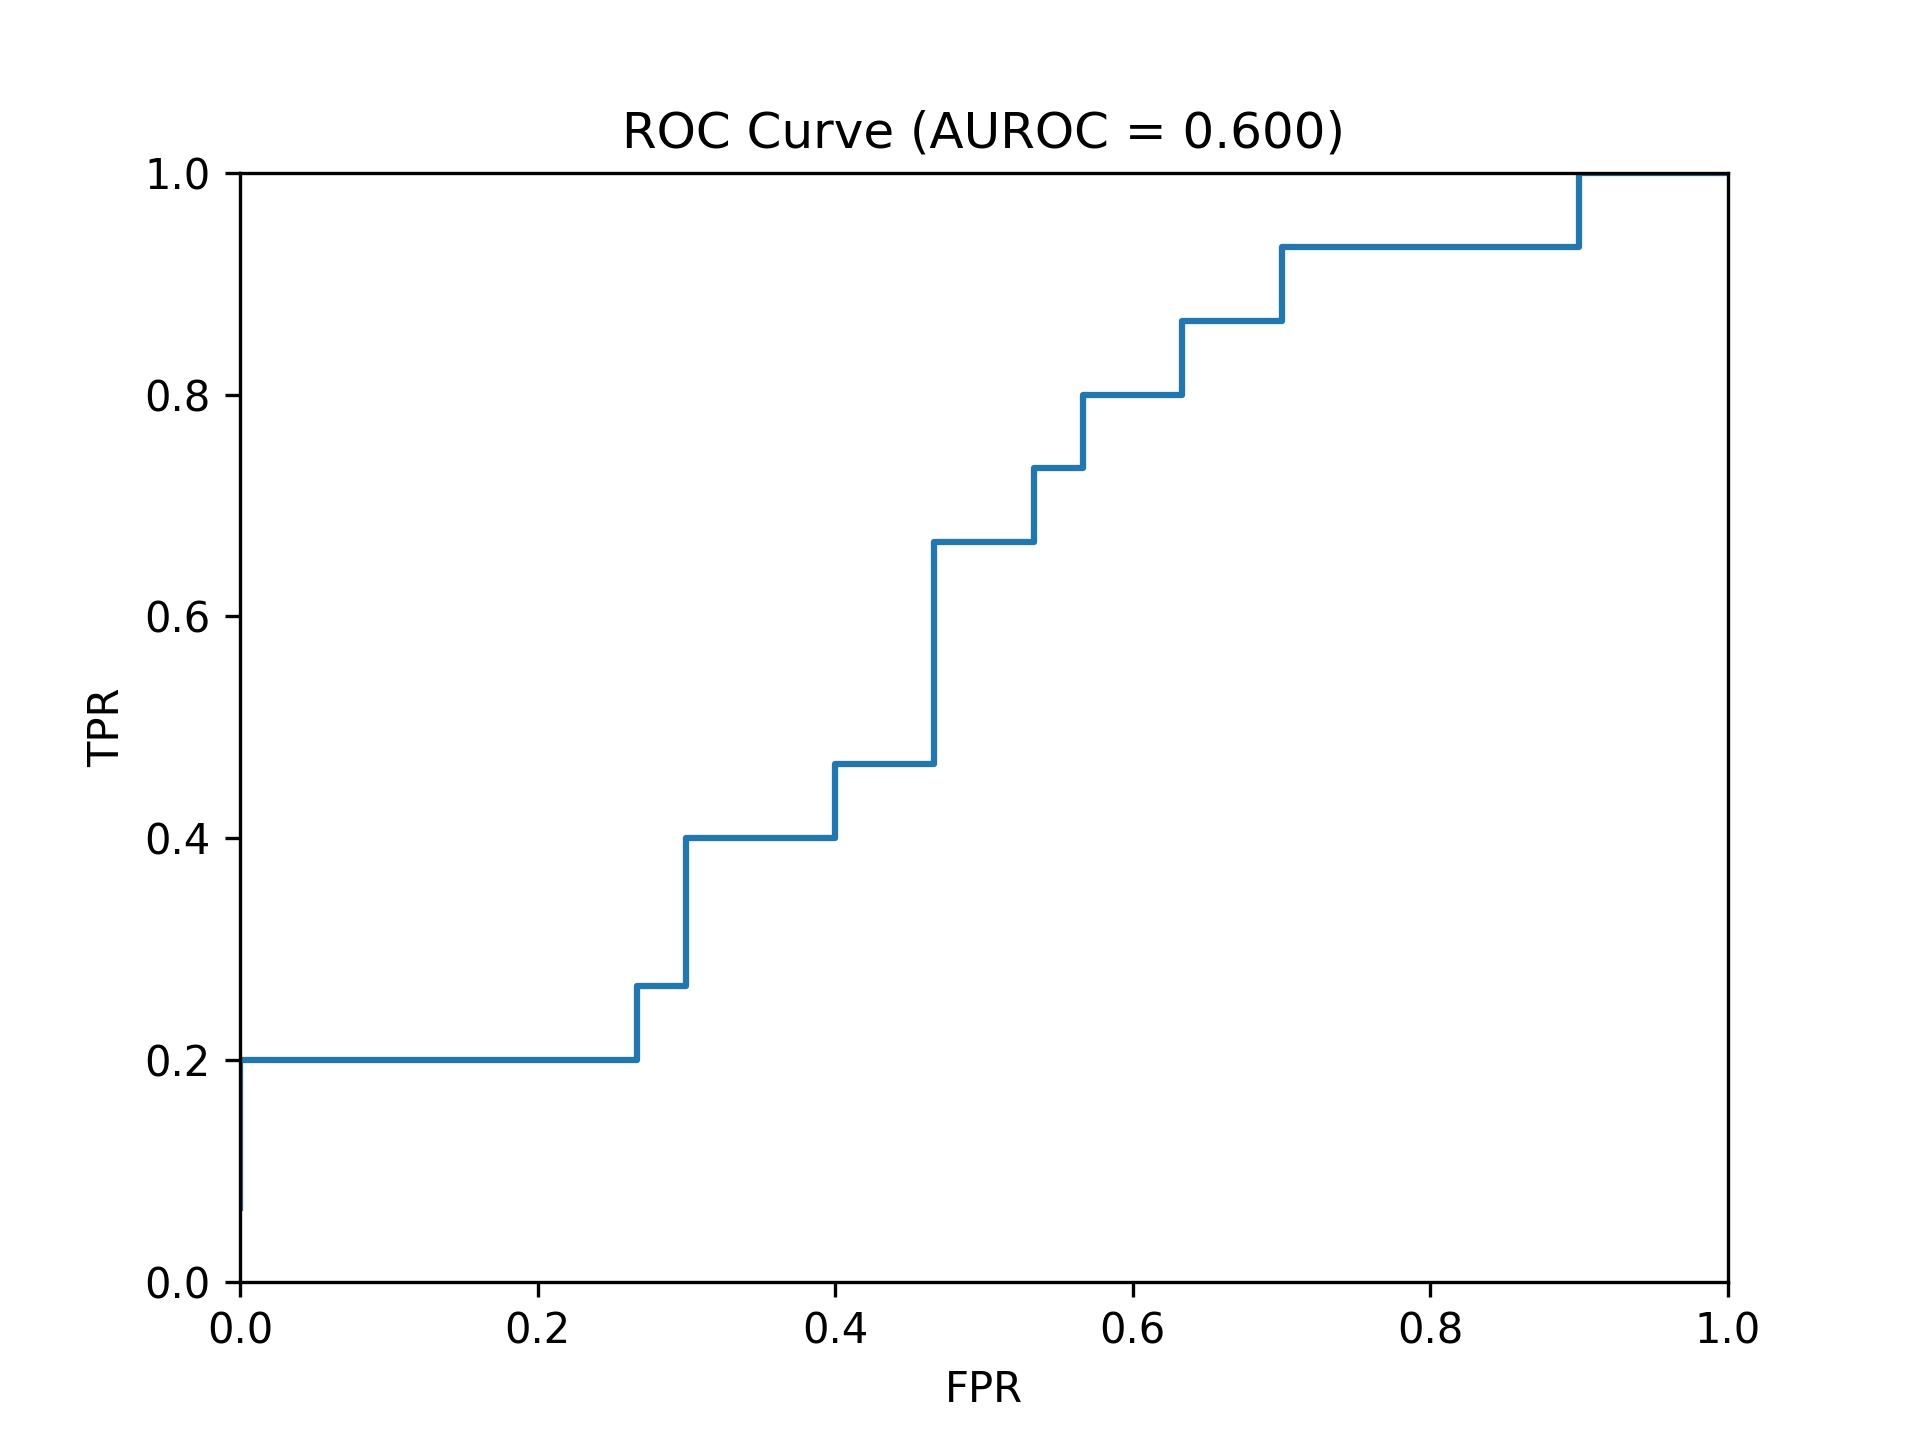
\includegraphics[width=3in]{den_9b.png} 
% \centering
% \end{figure}
%
%\begin{figure}[h!]
%\caption{Kernel Estimatiom}
% 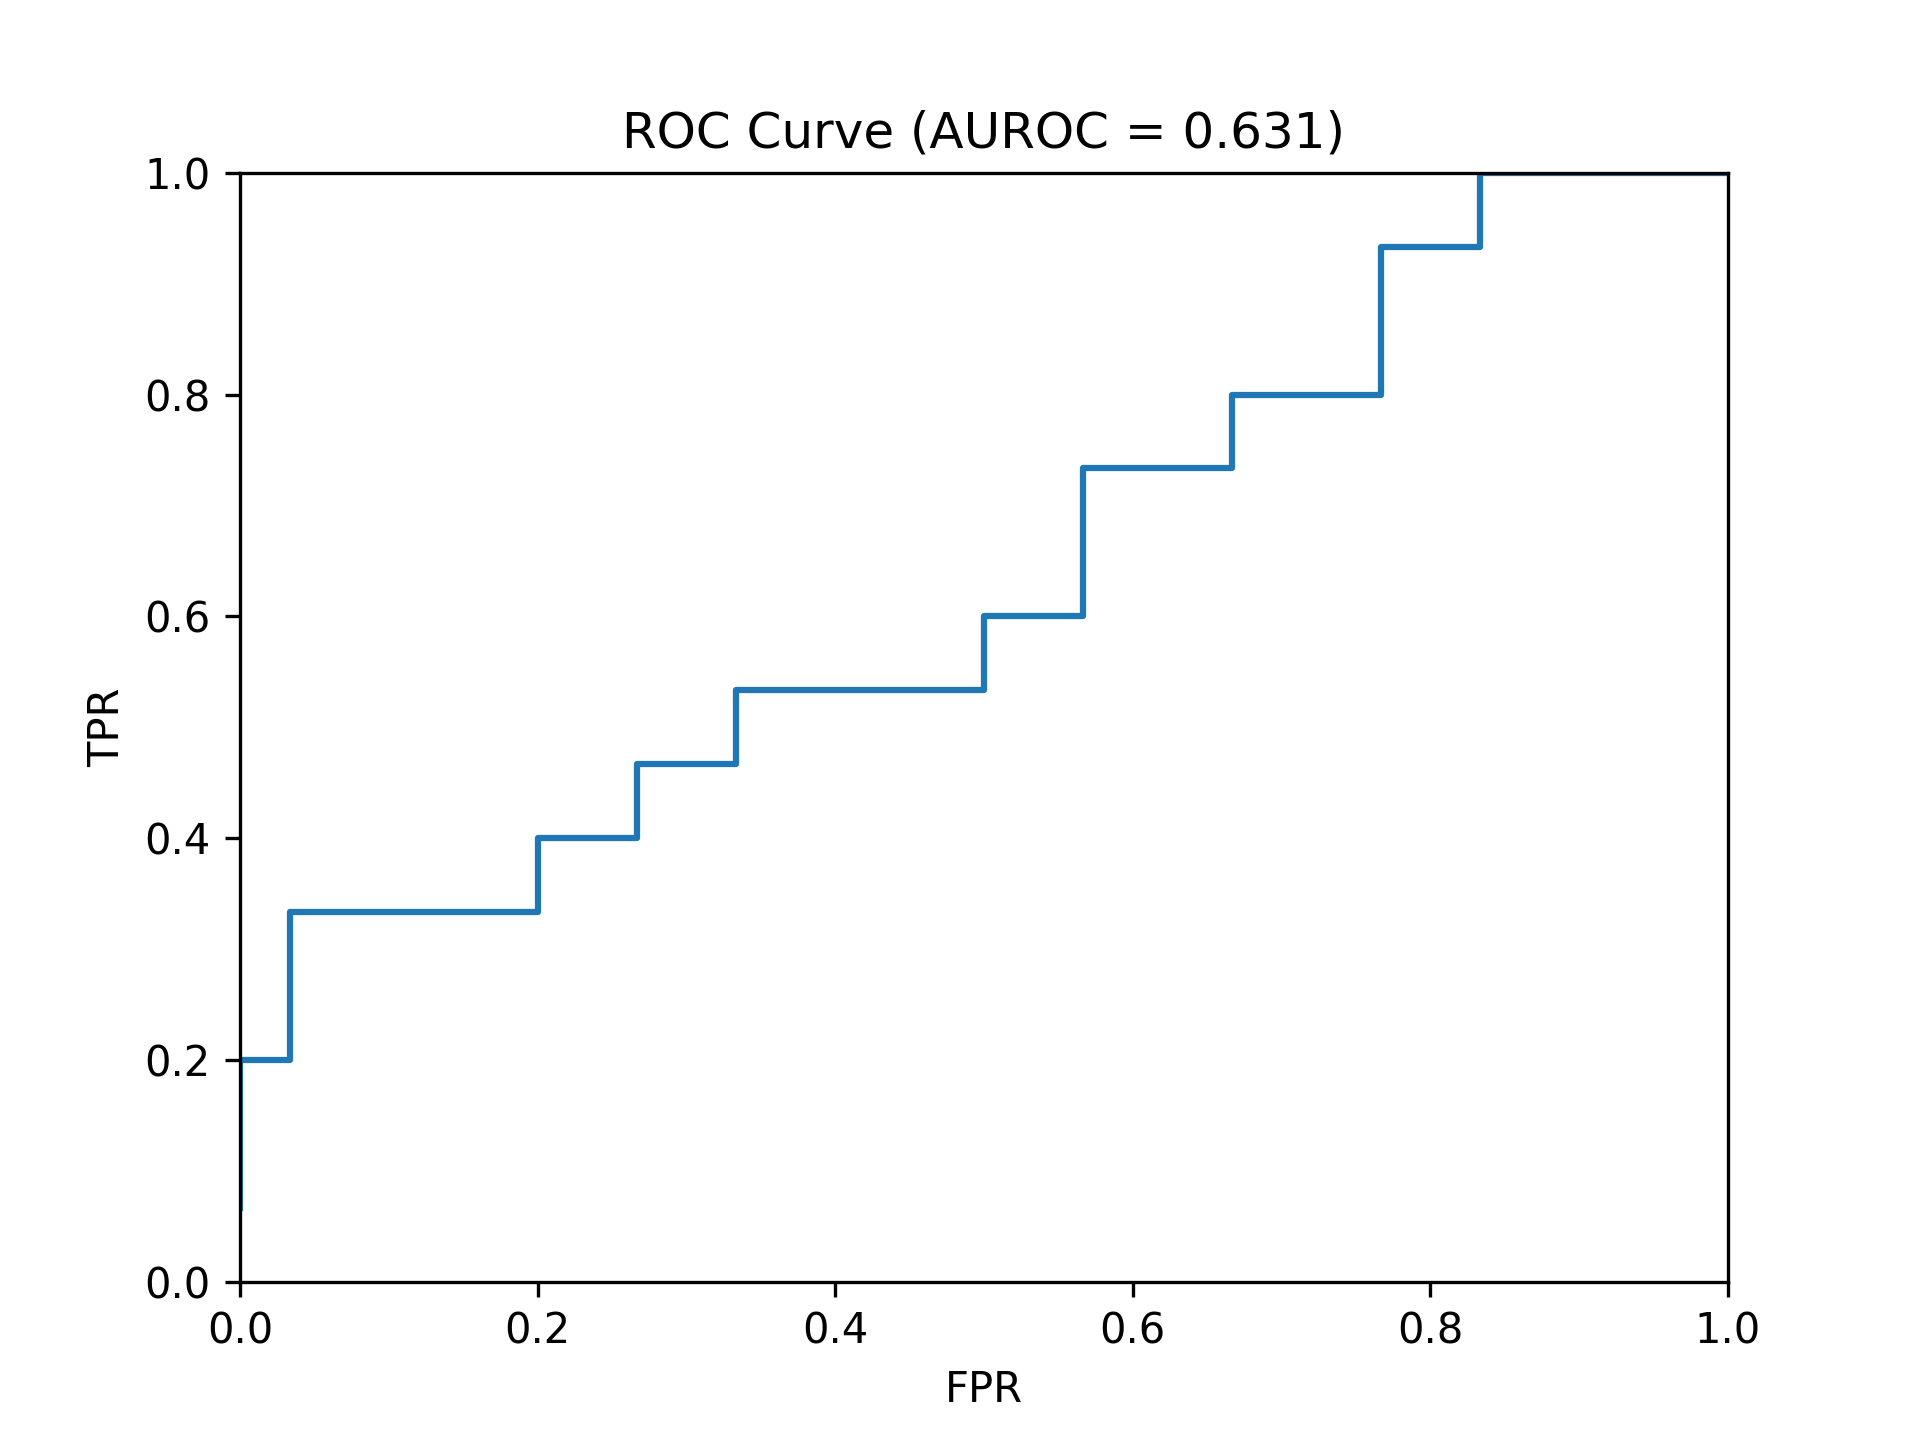
\includegraphics[width=3in]{kern.png} 
% \centering
% \end{figure}

%  \begin{algorithm}[]
%        \begin{algorithmic}[1]
%            \Function{OOPS\_exhausive}{$input\_seqs, W, \pi_{init}$}
%            	\State $bestProb = -\infty$
%		\For{W-mer in input\_seqs} 
%			\State $pwm \gets get\_init\_pwm(\text{W-mer})$
%			\State $Z,prob \gets E\_step\_get\_Z(pwm, sequences)$
%			\If {$ prob > bestProb$}
%				\State $best\_Z, best\_prob \gets Z, prob$
%				\State $best\_pwm \gets M\_step\_get\_pwm(Z,sequences)$
%			\EndIf
%			\State $pwm , Z \gets best\_pwm, best\_Z $
%	         \EndFor
%	         \While {not Converged}
%	         	\State $Z  \gets E\_step\_get\_Z(pwm, sequences)$
%			\State $pwm' \gets M\_step\_get\_pwm(Z,sequences)$
%			\State $Converged \gets |pwm'-pwm| <  tol$ 
%			\State $pwm \gets pwm'$
%	         \EndWhile
%            	\State{Write $pwm, Z_{i,max}, ...$} 
%            \EndFunction{}
%        \end{algorithmic}
%        \caption{Exhaustive Start OOPS Algorithm}
%    \end{algorithm}
%\end{homeworkProblem}
%
%\begin{homeworkProblem}
%\textbf{Motif Discovery}
%
%We suppose the input sequences in the file hw1\_hidden.txt come from the promoter regions of 100 yeast genes that
%are differentially expressed in a stress response experiment. We would like to use motif finding to learn more about a candidate regulator (transcription
%factor) of this expression response. Using our program from part I, we find the best OOPS motif of width 8:
%
%\begin{center}
% \begin{tabular}{|| c | c c c c c c c c c ||} 
%
% \hline
% ch & BG & Pos1 & Pos2 & Pos3 & Pos4 & Pos5 & Pos6 & Pos7 & Pos8 \\ [0.5ex] 
%  \hline 
%  C & 0.256 & 0.010 &  0.094 & 0.019 & 0.010 & 0.010 & 0.019 &  0.595 & 0.797 \\ 
% A & 0.241 & 0.240 & 0.010 & 0.022 & 0.970 & 0.856 & 0.020 & 0.251 & 0.010 \\
% G & 0.250 & 0.029 & 0.886 & 0.948 & 0.011 & 0.020 & 0.922 &  0.020 & 0.020 \\
% T & 0.252	& 0.721 &	0.010 & 0.011 & 0.010 & 0.114 & 0.040 &	0.135 & 0.174 \\ [1ex] 
%\hline
%\end{tabular} 
%\\[1.5ex]
%Hidden Motif PWM
%\end{center}
%
%\end{homeworkProblem}
%
%\pagebreak
%
%\begin{homeworkProblem}
%\textbf{Sequence Logo}
%
%    Express the PWM as a sequence Logo.\\[3pt]
%    
%   
\includegraphics[width=6in]{logo.pdf} 
%   
%\end{homeworkProblem}   
%
%\begin{homeworkProblem}
%\textbf{Transcription Factor Search}
%
%   To find a candidate match for our transcription factor, we go to JASPAR, "an open-access database of curated, non-redundant transcription factor (TF) binding profiles." By following the instructions on the alignment page, we see that the top hit, MA0304.1 (GCR1) is a very close match:\\[3pt]
%   
%   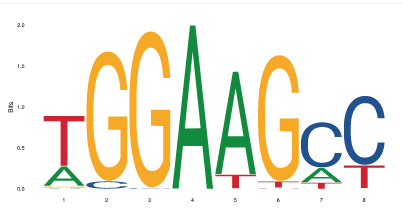
\includegraphics[width=4in]{MA0304_1.png} 
%   
%   Others in the top 5 include MA0377.1 (SFL1),  MA0305.1 (GCR2), MA0323.1 (IXR1), and MA0418.1 (YAP6), but they aren't nearly as close. The maximum possible score is 
%   two times the length of the two sequences, and the top hit was over 15, compared with 13 for second place. 
%   
%   There are slight differences. As the Jaspar description is "Finalized", it doesn't need to use pseudo counts, and thus the informational content is marginally higher at every location.
%   
%   Using the www.yeastgenome.org website, we find GCR1 is a "transcriptional activator of genes involved in glycolysis." From Wikipedia, glycolysis is the metabolic pathway that breaks down glucose into pyruvate, releasing the free energy needed to create the universal fuel ATP. GCR1 is known to regulate 86 genes. 
%  
%\end{homeworkProblem}   
%
%\begin{homeworkProblem}
%\textbf{ PWM Parameters}
%
%   
%    We are given the following motif solution, using no pseudocounts:
%    
%\begin{center}
%\begin{tabular} {| c |}
% \hline
% C\underline{\textbf{ATGT}}GAA \\
%CAG\underline{\textbf{CAGG}}G \\
%A\underline{\textbf{CCTC}}TTC \\
%\underline{\textbf{CAGA}}CATG \\
%AC\underline{\textbf{CTAT}}CG \\
%G\underline{\textbf{CGGC}}AGT \\
%\underline{\textbf{GTGT}}AGTT \\
%C\underline{\textbf{CAGG}}AAG \\
%AT\underline{\textbf{GACC}}GG \\
%GGA\underline{\textbf{TAGT}}A \\
%  \hline
%\end{tabular}
%\end{center}
%
%
%\begin{center}
%\begin{tabular}{ | c | c c c c | c |}
%\hline
%& i=1 & i=2 & i=3 & i=4 & Background \\
%\hline
%A & 0.1 &  0.5  & 0.1  & 0.1  & 0.325 \\
%C & 0.6  & 0.1 &  0.1  & 0.3  & 0.175 \\
%G &  0.2  & 0.1  & 0.7  & 0.2  & 0.325 \\
%T & 0.1 &  0.3  & 0.1  & 0.4  & 0.175 \\
%\hline
%\end{tabular}
%\end{center}
%
%\textbf{A) Extend existing solution to W = 5}\\[6pt]
%
%
%\begin{center}
%\begin{tabular}{ | c | c c c c c | c |}
%\hline
%& i=1 & i=2 & i=3 & i=4 & i=5 & Background \\
%\hline
%A & 0.100 & 0.500 & 0.100 & 0.100 & 0.400 & 0.300 \\
%C & 0.600 & 0.100 & 0.100 & 0.300 & 0.200 & 0.167 \\
%G & 0.200 & 0.100 & 0.700 & 0.200 & 0.300 & 0.333 \\
%T & 0.100 & 0.300 & 0.100 & 0.400 & 0.100 & 0.200 \\
%\hline
%\end{tabular}
%\end{center}
%
%\textbf{B) Compare Log Likelihoods}\\[6pt]
%
%
%\begin{center}
%\begin{tabular}{ | c | c |}
%\hline
%$\log_{10}P(X|W=4)$ & -42.73 \\
%$\log_{10}P(X|W=5)$ & -42.57 \\
%$\log_{10}P(X|W=5)- \log_{10}P(X|W=4)$ & 0.168 \\
%\hline
%\end{tabular}
%\end{center}
%
%\pagebreak
%
%\textbf{C) Discussion}\\[3pt]
%
%Extending the width will always give a likelihood which is greater than or equal to the shorter solution. \\[3pt]
%
%
%To see why, we can first look at the case in which $ W << L$, so background probabilities are unchanged by the single extension. Then the probability  of each character in each sequence will be unchanged, except for the terms in the $w+1$ motifs position. In the $W_0$ case, the background probabilities $p_{bg_c}$, are used, and in the $W_0 +1$ case, the probabilities used are the Dirichlet parameters, $p_{D_c}$,  calculated just for this position. The Dirichlet distribution was been shown to be a maximum likelihood estimator.  Thus 
%
%\[
%\prod_{c \in seqs_{W_0+1}}p_{D_c}  \ge \prod_{c \in seqs_{W_0+1}}p_{bg_c}
%\] 
%because it's greater than or equal for \textit{all} distributions. Therefore   
%
%\[
%	\frac{P(X|W=W_0+1)}{P(X|W=W_0)} = \prod_{c \in seqs_{W_0+1}}\frac{p_{D_c}}{p_{bg_c}} \ge 1
%\]\\[3pt]
%
%For the case in which the background changes, we note that the new background probabilities, 
%$p_{bg'_c}$ are again MLE estimators of all non-motif characters for the case in which the $W_0 +1$ characters \textit{are excluded}. 
%So their ratio is again greater than one:\\[3pt]
%
%\[
%	\prod_{c \notin \text{motif}_{W_0+1}} \frac{p_{bg'_c}} {p_{bg_c}} \ge 1
%\] 
%
%To complete the argument, we note when two terms that are each $ \ge 1$ are multiplied, their product is as well. This implies that while maximizing likelihood is able to find the best motif solution for a given width, it is not able to choose the \textit{best} width.
%
%\pagebreak
%
%\lstinputlisting[language=Python, caption=Problem 5 Code]{part5.py}
%
%\end{homeworkProblem}

\end{document}
